%APPENDIX B--TABLES AND GRAPHS
\newapp
%\section*{Data Handling}
%\addcontentsline{toc}{subsection}{Data Handling}
%\label{datahandle}
\section*{Tables}
     Experimental data are usually recorded in tabular
form (see Table~\ref{tableb2}).  The table should have labeled columns for the
both the independent and dependent variables.  Each column label should show
the units for that quantity.  A representative estimate of the
error should be made and recorded for the first entry in a column
and any other place that the value of the error changes
significantly.  (In this example the uncertainty in distance, $\delta S$,
and the uncertainty in time, $\delta t$, are the same for each
of the three data points; it is not uncommon to have varying uncertainties---
requiring a column just for uncertainty.  In addition if you are using a spreadsheet
to record values, enter numbers only, without the $\pm$.) Room for extra columns should be left if
quantities are going to be calculated from the direct
measurements.  A sample calculation should also be shown at the
bottom of the table for those quantities which are calculated.
\begin{table}[h]
\begin{center}
\begin{tabular}{|cll|}
\hline
point \# & $S$ (cm) & $t$ (sec) \\ \hline
1 & $0.00 \pm 0.05$ & $0.000 \pm 0.002$ \\
2 & $0.25$ & $0.016$ \\
3 & $0.71$ & $0.032$
\\ \hline
\end{tabular}
\end{center}
\caption{Sample distance and time data.  \label{tableb2}}
\end{table}
\begin{figure}    %linear graph of distance vs time
\begin{center}
{\resizebox{3.5in}{!}{\rotatebox{-90}{\includegraphics{appb_TB1.ps}}}}\hfill
\raisebox{-2.25in}{\resizebox{2.25in}{!}{{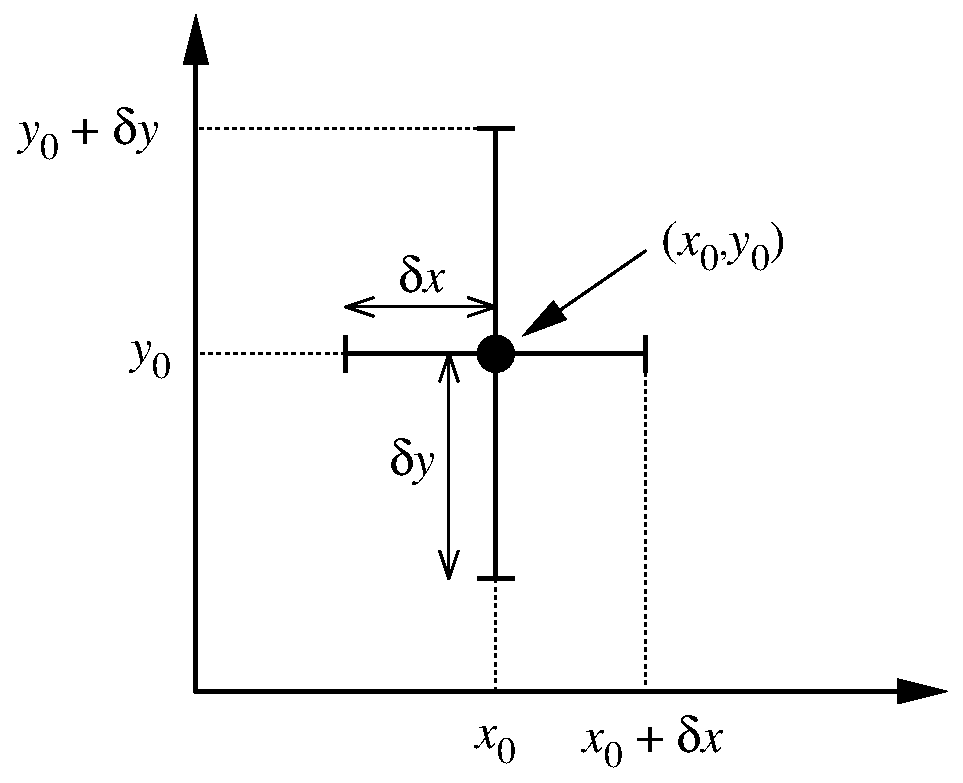
\includegraphics{errbarsB.eps}}}}
\end{center}
%\vspace{4in}
%\centerbmp{6.94in}{9in}{pressure.bmp}
%\special{ps:pressure.ps}
\caption{Plot of the data presented in Table~\protect\ref{tableb2} and
a typical graphed data point.  \label{fig:b1}}
\end{figure}

\section*{Graphs}
     Since it is much easier to recognize a pattern from a graph
(picture) than from a table, we will use graphs extensively in
this laboratory.  (The next Appendix, Graphical Analysis, will show you how to
recognize functional relationships from graphs.)

     Whenever possible, make an initial graph to monitor the experiment {\em as
you are collecting the data}.  As you record each measurement in a table,  plot it
on the graph.  After several points have been graphed, a pattern
(or shape) becomes apparent.  This pattern can then serve as a
general guide to tell whether subsequent measurements fit the
pattern.  Although we may not know the exact pattern the data
will follow, large deviations from any pattern can be easily
identified, thus catching problems in time to correct them.
This initial graph will also serve as the starting point for data
analysis.

     A final graph should always be included in your lab
write-up.  This graph should be a refined and more complete
version of your initial graph.  See Appendix C on Graphical Analysis for
several examples of properly prepared final graphs.  To insure that the
graphs give a clear picture of what is being represented, we ask
you to follow this set of rules:
%\begin{figure}[hbt]
%\begin{center}
%{\resizebox{3in}{!}{{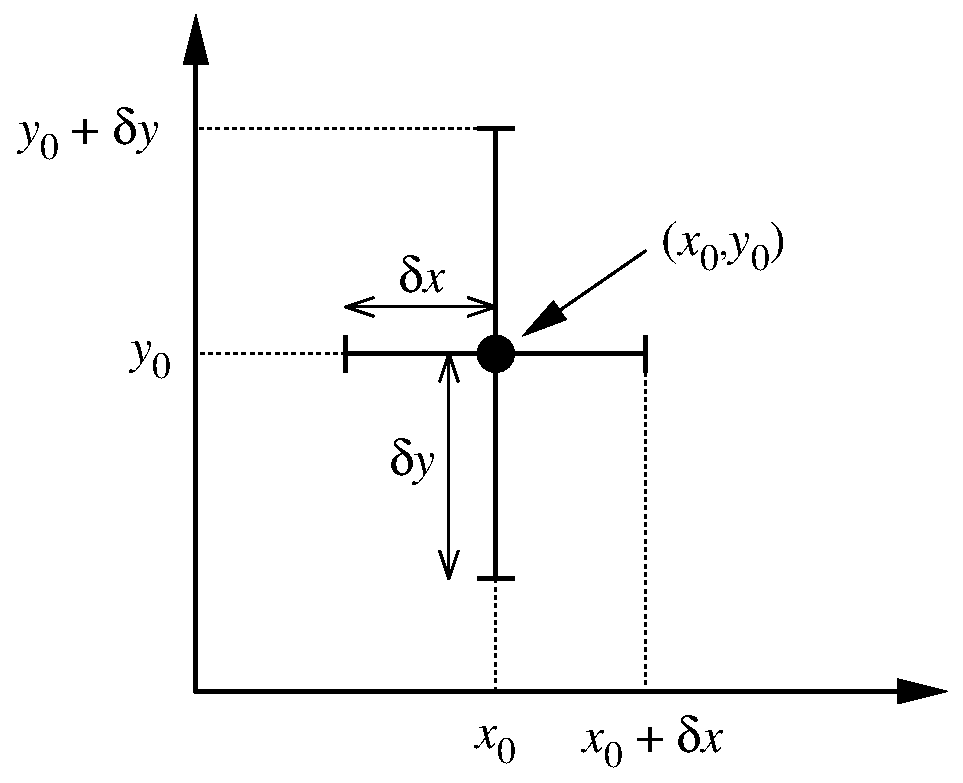
\includegraphics{errbarsB.eps}}}}
%\end{center}
%   \centerbmp{3.72in}{2.2in}{errbars.bmp}
% \caption{A typical graphed data point.  \label{fig:b1}}
%\end{figure}
\begin{enumerate}
\item Put a title on each graph in a place that will not
           obscure the data.
\item Label each axis with the name of the quantity and its
           units.
\item Select the graph scale such that the data spans most of
           a full page of graph paper --- {\em DO NOT} plot all of your
           data in one small section of the page!
\item On your final graph indicate the error in each graphed
           data point by using error bar symbols.
           An example of a typical graphed data point ($x_{\circ},y_{\circ}$)
           with error bars is shown in Fig.~\ref{fig:b1}.
           You need not show error bars that are smaller than the
           dot size.  However, note the fact that the errors are
           smaller than dot size below the graph's title.
\item {\bf Optional:}  With a pencil, lightly sketch a {\em smooth}
           curve through the data (do not play
           ``connect the dots'').  If this is an initial graph, the
           curve should represent your ``eyeball" approximation
           of the pattern.  For the final graph the smooth curve
           should be based upon your graphical or computer data
           analysis (as explained in the next two sections).
\end{enumerate}

